\documentclass[article]{uom-coursework}

% \usepackage{blindtext}
% \usepackage[showframe]{geometry}
\usepackage{float}
% \usepackage{listingsutf8}
\usepackage[backend=biber]{biblatex}

% \usepackage{syntax}
% \usepackage{mdframed}
% \usepackage[ruled]{algorithm2e}
% \usepackage[nopagecolor={white}]{pagecolor}
\usepackage{calc}

\usetikzlibrary{automata, positioning, arrows,
arrows.meta}

\def\CC{{C\nolinebreak\raisebox{.25ex}{\scriptsize\bfseries{++}}}}

\tcbuselibrary{most,documentation}

\tcbset{skin=enhanced,
  doc head={colback=yellow!10!white,interior style=fill},
  doc head key={colback=magenta!5!white,interior style=fill},
  doc head path={colback=blue!50!gray!7!white,interior style=fill},
  color key=DarkViolet,
  color value=Teal,
  color color=Teal,
  color counter=Orange!85!black,
  color length=Orange!85!black,
  index colorize,
  index annotate,
}

\newtcolorbox{note}[1][]{
  before skip balanced=2mm,after skip balanced=3mm,
  boxrule=0.4pt,left=5mm,right=2mm,top=1mm,bottom=1mm,
  colback=UMc8!50,
  colframe=UMc8!20!black,
  sharp corners,rounded corners=southeast,arc is angular,arc=3mm,
  underlay={%
    \path[fill=tcbcolback!80!black] ([yshift=3mm]interior.south east)--++(-0.4,-0.1)--++(0.1,-0.2);
    \path[draw=tcbcolframe,shorten <=-0.05mm,shorten >=-0.05mm] ([yshift=3mm]interior.south east)--++(-0.4,-0.1)--++(0.1,-0.2);
    \path[fill=UMc8!50!black,draw=none] (interior.south west) rectangle node[white]{\rotatebox{90}{\resizebox{!}{0.6em}{\bfseries NOTE}}} ([xshift=4mm]interior.north west);
    },
  drop fuzzy shadow,#1}

\newtcolorbox{noteline}[1][]{
  before skip balanced=2mm,after skip balanced=3mm,
  boxrule=0.4pt,left=5mm,right=2mm,top=1mm,bottom=1mm,
  colback=UMc8!50,
  colframe=UMc8!20!black,
  sharp corners,rounded corners=southeast,arc is angular,arc=3mm,
  underlay={%
    \path[fill=tcbcolback!80!black] ([yshift=3mm]interior.south east)--++(-0.4,-0.1)--++(0.1,-0.2);
    \path[draw=tcbcolframe,shorten <=-0.05mm,shorten >=-0.05mm] ([yshift=3mm]interior.south east)--++(-0.4,-0.1)--++(0.1,-0.2);
    \path[fill=UMc8!50!black,draw=none] (interior.south west) rectangle node[white]{\rotatebox{90}{\resizebox{!}{0.4em}{\bfseries NOTE}}} ([xshift=4mm]interior.north west);
    },
  drop fuzzy shadow,#1}



\addbibresource{dsa.bib}

\counterwithout{section}{chapter}

% Biblography
% \addbibresource{dsa.bib}

\title{Data Structures and\\Algorithms 2}
\tagline{Coursework}
\author{Juan Scerri}
\authorid{1234567A}
\courseworkname{Some Degree}
\doctype{coursework}
\courseworkdate{\monthyeardate\today}
\subjectcode{ICS2210}

\begin{document}

%----------------------------------
%	Front Matter
%----------------------------------

\pagestyle{umpage}

\frontmatter

\maketitle % Print the title page

\tableofcontents % Print the table of contents

\clearpage

\lstlistoflistings

\clearpage

\mainmatter

% \chapter{Report}

\chapter*{Report}
\label{chap:report}
\addcontentsline{toc}{chapter}{\nameref{chap:report}}

\section{Statement of Completion}

\begin{center}
\begin{tabular}{|l|l|} 
\hline
\textbf{Item} & \textbf{Completed (Yes/No/Partial)}\\
\hline
Created first array of integers & Yes \\
\hline
Knuth shuffle & Yes \\
\hline
Inserted in AVL tree & Yes \\
\hline
AVL tree insertion statistics & Yes \\
\hline
Inserted in Red-Black tree & Yes \\
\hline
Red-Black tree insertion statistics & Yes \\
\hline
Inserted in skip list & Yes \\
\hline
Skip list insertion statistics & Yes \\
\hline
Discussion comparing data structures & Yes \\
\hline
\end{tabular}
\end{center}

\section{Language}

The programming language used for this coursework is Python 3.
The main reason for this choice is the speed of development.

\section{Knuth Shuffling}

\lstinputlisting[caption={A function implementing Knuth shuffling.},language=Python,firstline=8,lastline=13]{../ics2210/knuth_shuffling.py}

Knuth shuffling, also known as Fisher-Yates shuffling, is an
algorithm used for generating permutations of the elements of a
given array.

The implementation follows the pseudocode described here in
\textcite{wikifisheryates}.

\section{Binary Search Tree}

First a Binary Search Tree (BST) was implemented. This is
because the basic structure of a BST underlies both
Adelson-Velsky-Landis (AVL) and Red-Black trees, helping reduce
code duplication.

The file \texttt{untyped\_tree.py} contains two of our base
building blocks. In particular these are \texttt{Node} and
\texttt{Tree}. As described the \texttt{Tree} class is a BST
with the main method being \texttt{insert()}. This is a basic
BST insert. Note however that a number of methods associated
with the Node class are being used.

Additionally, when creating a tree one can enable statistics to
keep track of the number of steps required for insertion to
complete.

Other methods required for collecting certain statistics
include: \texttt{calc\_height()} and \texttt{calc\_leaves()}.
They are quite self-explanatory, one is used to calculate the
height of the tree whilst the other is meant to calculate the
number of leaves the tree has.

The only issue with these methods is that they are recursive.
However, since the trees under consideration will be balanced
and are limited to 6000 nodes, they are well within the
recursion limit of the language. However, this is of course not
ideal and iterative approaches should be considered.

The \texttt{draw()} method, as its name implies, allows the
trees to be drawn and printed to the terminal. This method was
invaluable during development to ensure correctness of
algorithms by checking for parity with other implementations,
specifically those found at
\url{https://www.cs.usfca.edu/~galles/visualization/}.

If you wish to test the implementations for yourself, please use
\texttt{python} or \texttt{ipython}. Additionally, ensure that
you are in the root directory of the project. Then follow the
commands used in Figure \ref{fig:ipythonavl} and Figure
\ref{fig:ipythonskip}.

\begin{figure}[H]
\centering
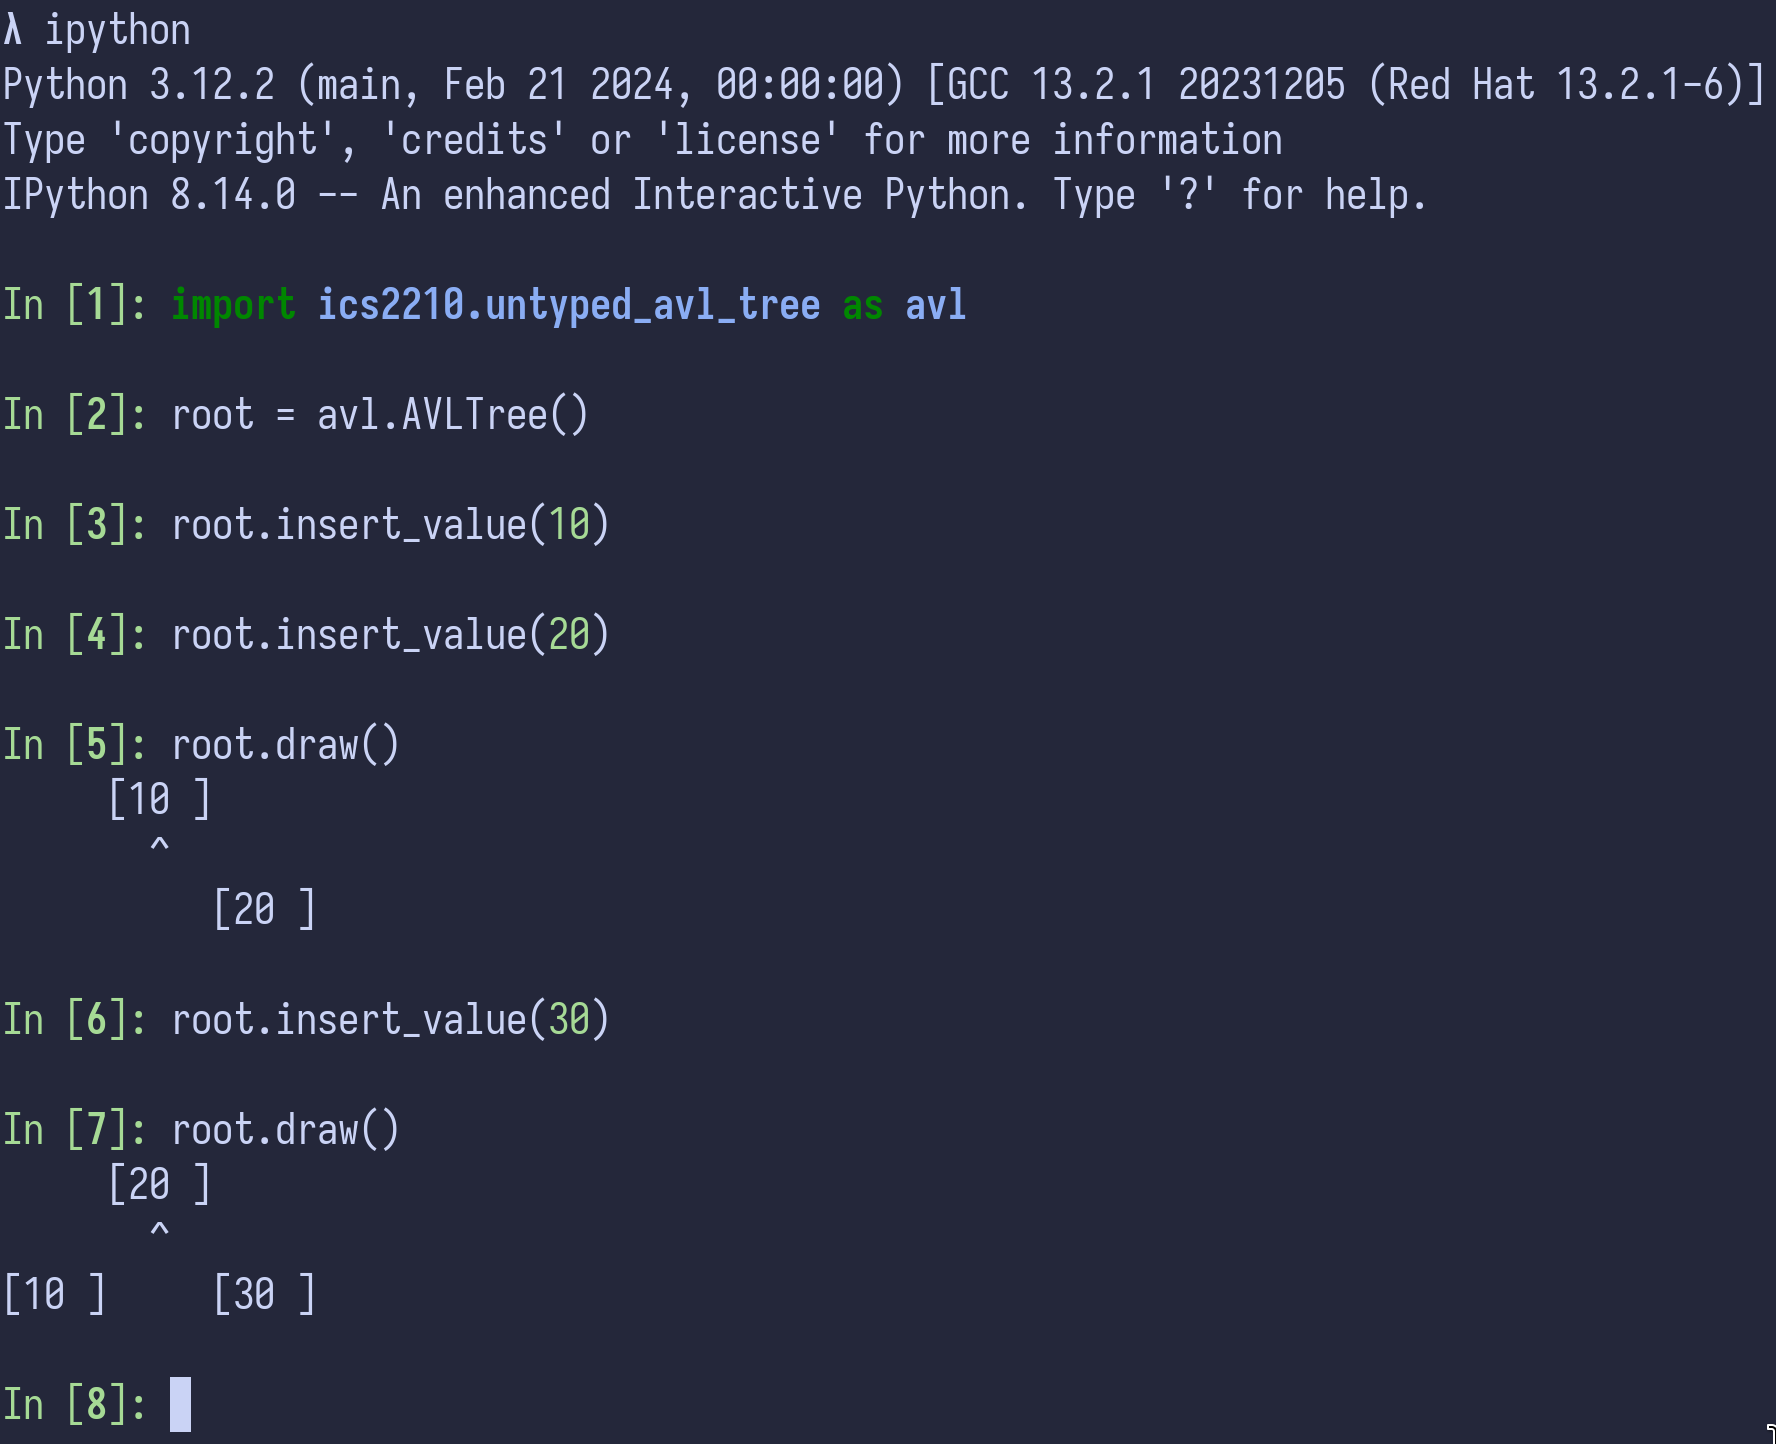
\includegraphics[width=\linewidth]{using-ipython-avltree.png}
\caption{Using an \texttt{AVLTree} (similar
interface for an \texttt{RBTree}).}
\label{fig:ipythonavl}
\end{figure}

\begin{figure}[H]
\centering
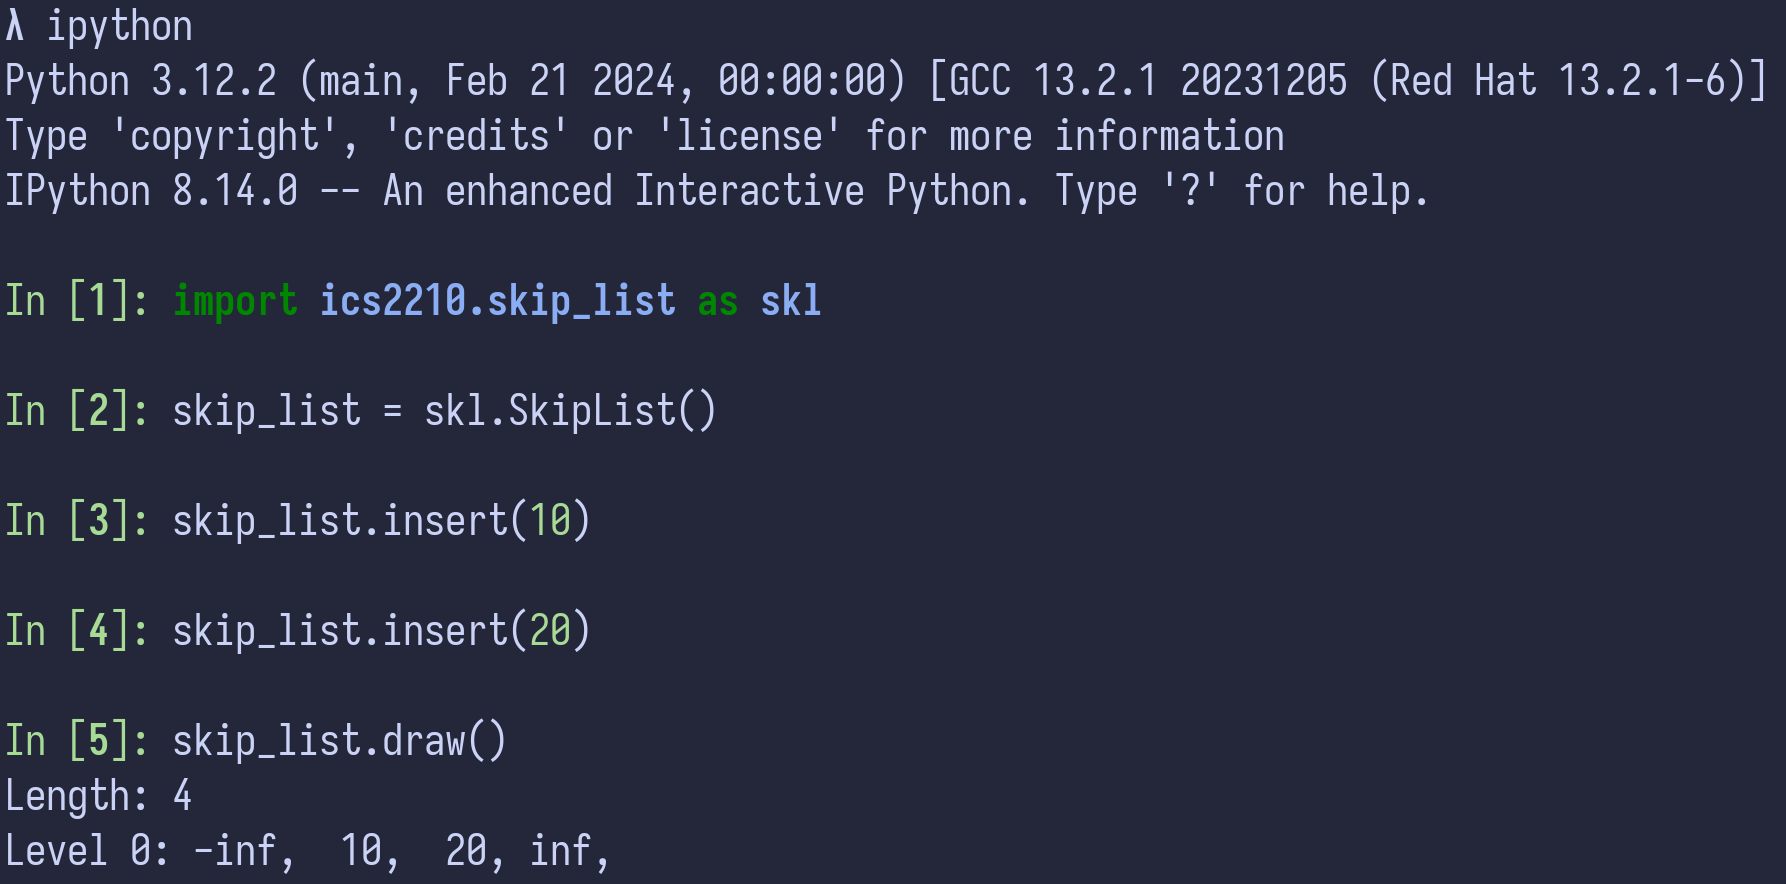
\includegraphics[width=\linewidth]{using-ipython-skiplist.png}
\caption{Using a \texttt{SkipList}.}
\label{fig:ipythonskip}
\end{figure}

Additionally, these classes have a baked in example which can be
run to test their behaviour (see Figure \ref{fig:example}).

\begin{figure}[H]
\centering
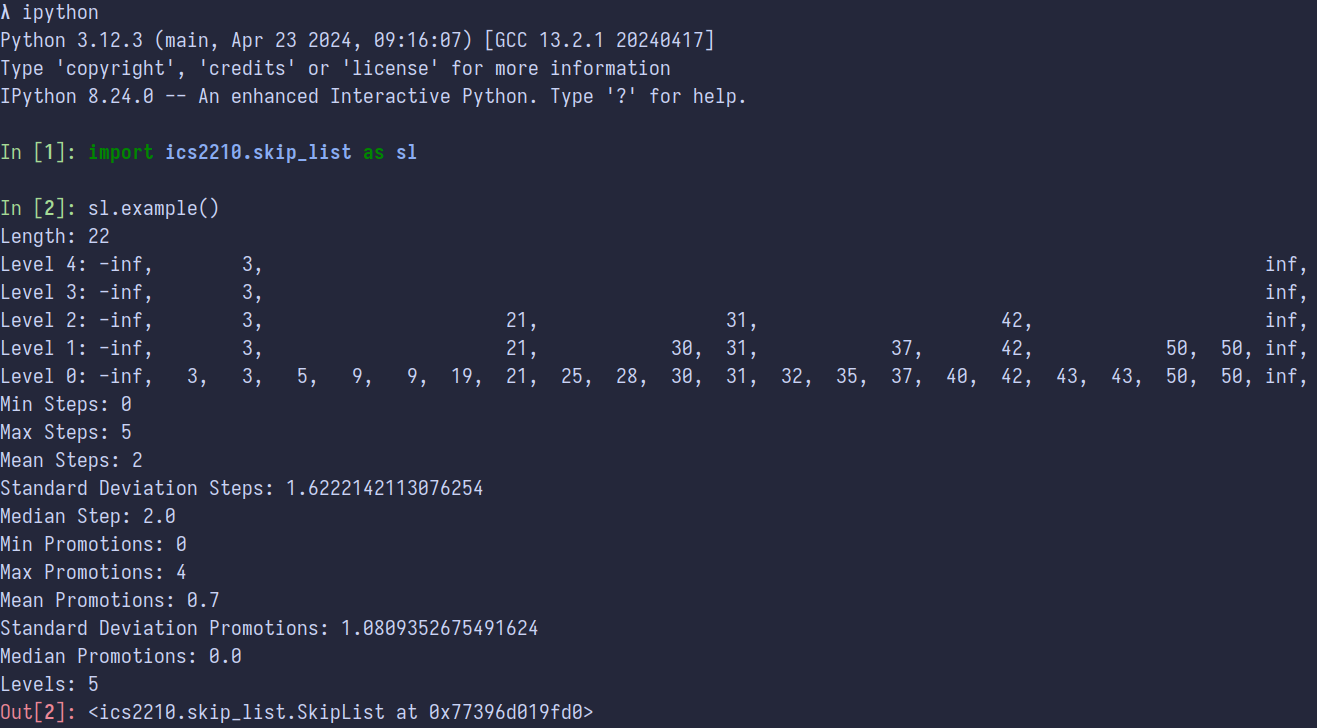
\includegraphics[width=\linewidth]{ipython-skiplist-example.png}
\caption{Using the builtin \texttt{SkipList} example (the
\texttt{AVLTree} and \texttt{RBTree} classes both also have a
builtin example).}
\label{fig:example}
\end{figure}

The \texttt{Node} class is a bit more complicated. It is not
simply a pure node. It contains a variety of methods which help
facilitate readable code within the encompassing data
structures, specifically the \texttt{AVLTree} and
\texttt{RBTree} classes.

The following methods are of particular interest:
\texttt{rotate()}, \texttt{can\_step()}, \texttt{value\_dir()}
and \texttt{dir()}. The other present method are fairly simple
and straight forward.

The \texttt{can\_step()} method returns a boolean indicating to
the callee whether or not a node has a child in the specified
direction.

The \texttt{value\_dir()} accepts a value which can be compared
with value present in the node. Then depending on whether the
value is greater than or less than the value in the node, a
direction is provided. In particular, if its is less than, the
\texttt{LEFT} direction will returned and if it is greater than
(or equal to) the \texttt{RIGHT} direction is returned.

\texttt{dir()} is used to check whether another node is on the
left or right of the current node.

\begin{note}
This method is \textbf{unsafe}. In particular if an other node
is provided and it is not a child of the self node then it will
be classified as being on the right of the node which is of
course incorrect.
\end{note}

The \texttt{rotate()} method was inspired by the
\texttt{RotateDirRoot()} function in \textcite{wikirbtree}. It
is a simple method which generalises LL and RR rotations. The
benefit of this is that LR and RL are just composition of LL and
RR rotations. Hence, complexity within the code for AVL trees
and Red-Black trees is reduced because there is no need for
thought about the actual mechanism for rotation.

\section{AVL Trees}

AVL trees were implemented by first inheriting from the base
classes described above. The \texttt{left\_height} and
\texttt{right\_height} fields were added as they are required
for rebalancing. Additionally, the \texttt{height\_diff()}
method allows for the calculation of the difference in height
between the left and right sub-trees of \texttt{self} i.e. that
specific \texttt{AVLNode}. The \texttt{update\_heights()} method
is used in the event that the tree requires rebalancing directly
afterwards to ensure correct heights.

\begin{lstlisting}[caption={The main insert function for AVL trees},language=Python]
def insert(self, node):
    self.root = self.fix(super().insert(node))
\end{lstlisting}

The \texttt{fix()} method rebalances the tree after an
insertion, if required. It is mostly an intuitive implementation
of the algorithms as they would be described on a piece of
paper.

In particular, the method starts from the inserted node, and
checks that each node in the path up to the root is balanced. If
not, one of the rebalancing algorithms LL, LR, RR or RL is
employed.

\begin{note}
At the end, the root is returned. This is critical because the
root of the tree can change due to rotations.
\end{note}

The code is additionally sprinkled with bits and pieces which
keep track of the necessary statistics. This is acheived by
using the the fact that if-statements in \texttt{python} do no
create a scoped of their own.

\section{Red-Black Trees}

Similarly, as discussed for AVL trees, the \texttt{RBNode} and
\texttt{RBTree} classes inherit from their respective bases
classes. The \texttt{RBNode} class has two additional methods,
\texttt{sibling\_is\_red()} and \texttt{get\_sibling()}.

\begin{note}
Both methods assume that the \texttt{self} node has a parent and
hence a sibling (if the left/right node is \texttt{None} it is
considered as a black node).
\end{note}

The \texttt{RBTree} class similarly to the \texttt{AVLTree}
class has a \texttt{fix()} method. The \texttt{fix()} method
again starts at the inserted node and traverse up to the root,
at each step checking for colouring violations and fixing them
if necessary. 

\begin{note}
The \texttt{fix()} for a Red-Black tree does not need to
traverse up the whole tree to the root. If at any point, a
non-black parent is reached, insertion is complete.
\end{note}

Again, a similar approach to collecting statistics is used.

\section{Skip Lists}

Before implementing a skip list, an extended integer class was
defined. In particular, the set of objects instantiated by the
class is the set of all integers and the objects `$-\infty$' and
`$\infty$'. Of course,kkkjjj the most natural property these objects,
which are called ``infinity'', have is the following:

$$\forall z \in \mathbb{Z} \cup \{-\infty, \infty\}, -\infty \leq z \leq \infty$$

The main reason for the inclusion of this type is to facilitate
a more natural implementation. In particular, this helps avoid
issues with not having a top-most left element.

\begin{figure}[H]
\centering
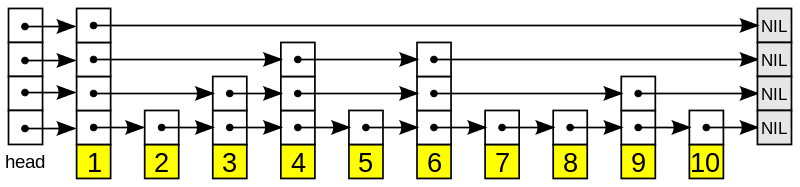
\includegraphics[width=\linewidth]{wikipedia-skip-list.png}
\caption{A graphical depiction of a skip list (source: \url{https://en.wikipedia.org/wiki/File:Skip_list.svg}).}
\label{fig:imageskiplist}
\end{figure}

Figure \ref{fig:imageskiplist} was a great inspiration and
helped to guide the implementation of the skip list. Each
element in a skip list is an instance of the \texttt{SkipNode}
class and each skip node is a value and a list or array
(whichever one \texttt{python} uses under the hood) of pointers.

The \texttt{SkipNode} class has two class methods which generate
the head and tail nodes respectively. Along with an
\texttt{add\_level()} method which increases the size of the
associated list or array by one. The \texttt{add()} method
allows the addition of a new skip node in between \texttt{self}
and the next skip node at a specified level.

Finally, the skip list itself keeps track of the head and tail
of the list along, with the height and length. Additionally, if
enabled, the specified statistics will also be collected.

The \texttt{insert()} method is the primary method in the
\texttt{SkipList} class. In particular, it traverses the skip
list, keeping track of all the nodes which contain the largest
value less than, or equal to the value being inserted. These
values are kept in a stack as the algorithm traverses down the
list.

Keeping track of these nodes is important for the second phase
of the insertion algorithm. After inserting in the lowest level,
a node can be promoted a random number of times. As the node is
promoted, it needs to be linked with the appropriate skip nodes
at its current level. It is important that it is linked to the
correct skip nodes to maintain the ordering of the skip list.
This is facilitated by the stack described above.

\section{The \texttt{procedure.py} File}

This file contains the steps described within the coursework
specification. The requirements for running the file are present
within the \texttt{README.md} file. To reiterate please ensure
that a \texttt{python} version greater than or equal to
\texttt{3.11.8} is installed. 

\begin{noteline}
Other versions of \texttt{python} have \textbf{not} been \textbf{tested}.
\end{noteline}

Since the \texttt{procedure.py} file has been marked by a
\texttt{\#!/usr/bin/env python3} and made executable, it can be
run with the following \texttt{./procedure.py} in a terminal.
Ensure that when doing so you are in the root directory of the
project. Additionally, if that does not work it can be run with
\texttt{python3 procedure.py}, again from the root directory.

\section{Discussion}

Running \texttt{./procedure.py} yields the following result:\label{list:stats}

\begin{lstlisting}[escapeinside={(*@}{@*)}]
(*@\char"03BB@*) ./procedure.py 

--- Inserting the first 5000 integers! ---

AVL Tree Stats:
Min Steps: 0
Max Steps: 13
Mean Steps: 10.064412882576516
Standard Deviation Steps: 1.6623348499094164
Median Step: 10
Min Rotations: 0
Max Rotations: 1
Mean Rotations: 0.4632
Standard Deviation Rotations: 0.4986937929228917
Median Rotations: 0.0
Height: 14
Leaves: 2143

RB Tree Stats:
Min Steps: 0
Max Steps: 14
Mean Steps: 10.089017803560711
Standard Deviation Steps: 1.6675100153653153
Median Step: 10
Min Rotations: 0
Max Rotations: 1
Mean Rotations: 0.38947789557911583
Standard Deviation Rotations: 0.4876806746608557
Median Rotations: 0
Height: 14
Leaves: 2146

Skip List Stats:
Min Steps: 0
Max Steps: 29
Mean Steps: 9.3812
Standard Deviation Steps: 4.051711963351639
Median Step: 9.0
Min Promotions: 0
Max Promotions: 14
Mean Promotions: 1.0266
Standard Deviation Promotions: 1.462983425777893
Median Promotions: 0.0
Levels: 15

--- Inserting the other 1000 integers! ---

AVL Tree Stats:
Min Steps: 0
Max Steps: 14
Mean Steps: 10.461576929488247
Standard Deviation Steps: 1.7923596452927255
Median Step: 11
Min Rotations: 0
Max Rotations: 1
Mean Rotations: 0.4676666666666667
Standard Deviation Rotations: 0.498995044963413
Median Rotations: 0.0
Height: 14
Leaves: 2575

RB Tree Stats:
Min Steps: 0
Max Steps: 15
Mean Steps: 10.513085514252376
Standard Deviation Steps: 1.8388168878486906
Median Step: 11
Min Rotations: 0
Max Rotations: 1
Mean Rotations: 0.39006501083513917
Standard Deviation Rotations: 0.4878052518805189
Median Rotations: 0
Height: 15
Leaves: 2574

Skip List Stats:
Min Steps: 0
Max Steps: 29
Mean Steps: 10.216666666666667
Standard Deviation Steps: 4.417915257006624
Median Step: 10.0
Min Promotions: 0
Max Promotions: 14
Mean Promotions: 1.02
Standard Deviation Promotions: 1.4467027423780374
Median Promotions: 0.0
Levels: 15
\end{lstlisting}

\subsection{The Oneness of Balanced Trees}

A particularly interesting observation is the strange outcome
that after 6000 insertions both AVL trees and Red-Black trees
only ever use at most one rotation to rebalance. This is by no
means an oddity. As mentioned in \textcite{wikirbtree}, the
`Noted to the insert diagrams' section, specifically the last
bullet point and in \textcite{wikiavltree}, the `Delete'
section, specifically the third paragraph, this is expected
behaviour. Within the above web-articles they are specified as
incurring at most two rotations, however, in our implementation
an LR or RL rotation, although composed of two successive
rotations, is considered as one rotation.

\subsection{Balanced Trees vs.\ Skip Lists}

The time complexity of skip lists is probabilistically identical
to AVL and Red-Black trees. This means that the effectiveness of
a skip list is dependent on whether or not its source of
randomness is truly random or not. Most pseudo-random number
generators will probably have a bias and that bias needs to be
tested to ensure that the tolerances are good enough to
guarantee the time-complexities that a skip list advertises.

This means that the environment in which a skip list will
operate will most certainly determine its effectiveness. A
particularly well-suited example would be a memory constrained
environment. This is because the size of a skip list in terms of
the of instruction count is significantly smaller than that of
an AVL or Red-Black tree.

However, this will still require researching and benchmarking
the performance of a skip list. This can be done by using a
number of data sets and by measuring the bias introduced by the
random number generator.

It is also crucial to point out that all three different data
structures are not very cache friendly. This is because
cache-hit rate optimisation is hard for non-contiguous data
structures such as the ones under consideration.

Of course, skip lists and the trees are fundamentally different
types and hence they might exhibit different cache
characteristics but none will ever be as cache-friendly as a
fixed size array.

A slight note on thread-safety: as mentioned in this post on
\url{https://stackoverflow.com/questions/256511}, locking
locality can be a consideration. In particular, skip list can be
easily augmented to support multithreaded insertion. This is
because for every insertion, a skip list only needs to lock the
two neighbouring skip nodes. However, there do seem to exist
lock-free Red-Black tree implementations.

Moreover, the tree-based algorithms are guaranteed to give the
performance they advertise. This is because
their worst-case complexity for all types of operations
is $O(\log n)$.

Additionally, as indicated by the standard deviation of the
number of steps required to reach the adequate insertion
position, a skip list has higher levels of variation due to its
probabilistic nature. This indicates a more uniform access time
for AVL and Red-Black trees.

As a final verdict, when operating on normal general purpose
computers, it is more appropriate to choose a tree-based data
structure. Not only do modern computers have a enough memory to
load the instructions required to implement AVL trees or
Red-Black trees, but using a tree-based algorithm provides a
non-probabilistic bound on the worst-case time-complexity.
Hence, a skip list should be considered only when necessary.

\subsection{AVL Trees vs.\ Red-Black Trees}

Now that trees vs.\ skip lists has been discussed, AVL trees
vs.\ Red-Black trees will be discussed.

\begin{figure}[H]
\centering
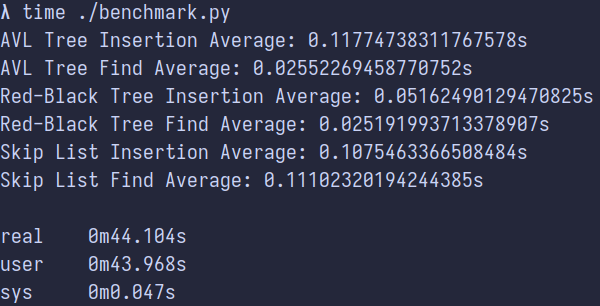
\includegraphics[width=\linewidth]{benchmark.png}
\caption{A benchmark calculating the average amount of time in
seconds it takes to insert 10000 elements and find 10000 times
for each data structure (on a single-thread as fast as
possible).}
\label{fig:benchmark}
\end{figure}

\begin{figure}[H]
\centering
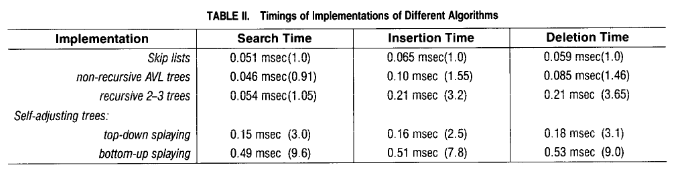
\includegraphics[width=\linewidth]{table2-pugh.png}
\caption{A figure of Table 2, as presented in \textcite{pugh90}.}
\label{fig:test9}
\end{figure}

In particular in \textcite{pugh90}, specifically table 2, the
author claims that AVL trees have an insertion time roughly
twice as slow as skip lists. However, according to the benchmark
in Figure \ref{fig:benchmark}, this is actually not the case. In
fact, AVL trees might actually be faster since the
implementation used for this coursework does not stop early when
inserting.

However, this might just be a matter of implementation. What
matters is that this pushes the discussion in an interesting
direction regarding, AVL trees and Red-Black trees.

AVL trees, as mentioned in \textcite{wikiavltree} are
more strictly balanced than Red-Black trees, making
them more ideal for searching-intensive applications.

Having said that, the benchmark and statistics indicate that on
average Red-Black trees almost have the same height as AVL trees
(see Listing in Section \ref{list:stats} and Figure
\ref{fig:benchmark}). This means that in scenarios where no hard
requirement on search speed is imposed, both AVL trees and
Red-Black trees perform well.

What pushes Red-Black trees over AVL trees is the fact that
insertion is seemingly twice as fast. It is possible that this
is the case because during `fixing', the algorithm can terminate
when it reaches a black parent. This means that unlike the AVL
tree implementation which traverses all the way up to root, the
Red-Black tree implementation terminates early. Additionally,
this speed up is more pronounced due to the fact that during
testing Red-Black trees were capable of maintaining a similar
height to AVL trees.

\section{Conclusion}

Red-Black trees seem to be the most natural choice for a data
structure with $O(\log n)$ time-complexity for all three types
of operations, in the most general of environments. It only
makes sense to use skip lists or AVL trees under the previously
discussed scenarios. 

Additionally, there are multiple examples of Red-Black trees
being used instead of AVL trees or skip lists. This because
Red-Black trees have better overall general characteristics.

Some of the above mentioned examples are: the \CC{}
\texttt{std::set} type, extensive use within the Linux kernel
(see \url{https://www.kernel.org/doc/Documentation/rbtree.txt})
and probably many many more.

\printbibliography

\end{document}
